\documentclass[12pt, letterpaper]{article} % [Tamano de la fuente, Tamano del papel]

% Tamano de la pagina y margenes.
\usepackage[letterpaper,top=2cm,bottom=2cm,left=3cm,right=3cm,marginparwidth=1.75cm]{geometry}

% packages utiles
\usepackage{amsmath}
\usepackage[colorlinks=true, allcolors=blue]{hyperref}
\usepackage{graphicx}
\graphicspath{{imagenes\}}} % Direccion de las imagenes
\usepackage{listings}

% Informacion del documento
\title{Colecciones en Java}
\author{Equipo 11}
\date{¿? de Octubre de 2022}

% Texto del documento
\begin{document}
\maketitle % Permite la apacion de la informacion del documento

% Nota Negritas: \textbf{greatest}
%      Subrayar: \underline{science} 
%      Cursiva: \textbf{\textit{accident}}

\textbf{Integrantes:}
\begin{itemize}
    \item Alfaro Dominguez Arturo.
    \item Herrera Lezama Fabricio Daniel.
    \item Lopez Gonzalez Erick.
\end{itemize}

\section*{¿Que son las colecciones?}
Las colecciones representan un grupo de objetos, estos objetos son conocidos como elementos, cuando se necesita trabajar con un conjunto de elementos, se necesita de un contenedor o almacen para guardarlos. En Java se proporciona la interfaz Collection, dicha interfaz permite almacenar cualquier tipo de objeto, como tambien, es posible usar ciertos metodos para su manipulacion, tales como: anadir, eliminar, conocer el tamano de la coleccion, etc. 

\section*{¿Que es un marco de recopilacion de Java?}

Un marco de recopilacion de Java proporciona una arquitectura para almacenar y manipular un grupo de objetos. Un marco de recopilacion de Java incluye lo siguiente:

\begin{itemize}
    \item \textbf{Interfaces:} Una interfaz en Java se refiere como tal a los tipos de datos abstractos, permitiendo manipular las colecciones de Java independientemente de los detalles de su representacion. Como tambien, forman una jerarquia en los lenguajes de programacion con el paradigma orientado a objetos.
    \item \textbf{Clases:} Las clases para Java son la implementacion de la interfaz de coleccion, es decir, las estructuras de datos que se utilizan.
    \item \textbf{Algoritmo:} Se refiere a los metodos que utilizan para realizar operaciones como busqueda y clasificacion en objetos que se implementan en las interfaces de coleccion.
\end{itemize}

El marco de recopilacion de Java proporciona a los desarrolladores el acceso a estructuras de datos pre empaquetadas, asi como a algoritmos para manipular datos.

\section*{Modelo de la jerarquia de colecciones en Java}
En el paquete de utilidades de Java (java.util) contiene todas las clases e interfaces que requiere el marco de la coleccion. El marco de la coleccion contiene una interfaz denominada interfaz iterable que proporciona el iterador para iterar a traves de todas las colecciones. Esta interfaz se amplia con la interfaz de recopilacion principal, que actua como raiz del marco de recopilacion. Todas las colecciones amplian esta interfaz de coleccion ampliando asi las propiedades del iterador y los metodos de esta interfaz.

A continuacion se presenta el diagrama que ilustra la jerarquia de colecciones en Java:
\begin{figure}[h]
    \centering
    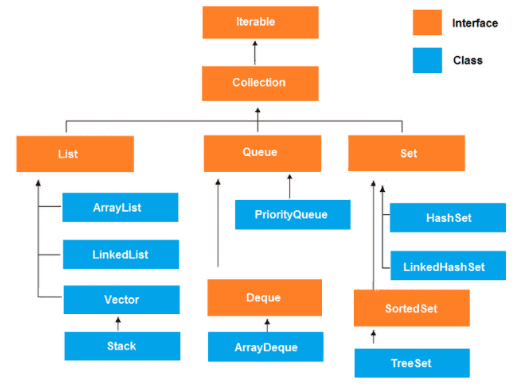
\includegraphics[width=0.75\textwidth]{imagenes/Jerarquia de colecciones Java.png}
    \caption{Pie de pagina.}
    \label{fig:jerarquia}
\end{figure}

Con el diagrama presentado, podemos observar cada una de las interfaces y clases que se conforman en dicha jerarquia. Como siguiente se procedera a explicar en detalle  las clases presentadas, sus metodos principales, sus diferencias entre ellas y los aspectos mas relevantes al momento de elegir alguno de ellos.

\section{Colecciones de Java: Lista (List)}
Para el apartado de la lista, tenemos que una lista es una coleccion ordenada de elementos que pueden contener en ellos elementos duplicados. Es una interfaz que amplia la interfaz de coleccion, dichas listas se clasifican ademas en lo siguiente:

\begin{enumerate}
    \item Lista de arreglo (Array List)
    \item Lista enlazada (Linked List)
    \item Vectores (Vector)
\end{enumerate}


\section*{Lista de arreglo (Array List)}
Lista de arreglo o Array List es la implementacion de List Interface donde los elementos se pueden agregar o eliminar de forma dinamica en la lista. A su vez, el tamano de la lista aumenta dinamicamente si los elementos se agregan mas que el tamano que posee en un inicio.

\begin{figure}[h]
    \centering
    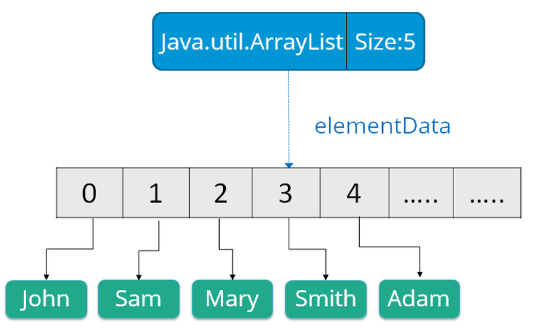
\includegraphics[width=0.75\textwidth]{imagenes/Ejemplo Grafico ArrayList.png}
    \caption{Pie de pagina.}
    \label{fig:ejemploarraylist}
\end{figure}

\section*{Forma para crear un Array List}
Se debe tomar en cuenta que para su creacion se debe importar la biblioteca:

\begin{center}
    import java.util.ArrayList;
\end{center}

A continuacion se presenta la forma para declarar un ArrayList:
\begin{center}
    \(ArrayList<Tipo de dato]> [Identificador] = new ArrayList<Tipo de dato]>(Tamano);\)
\end{center}

Donde se tiene que:
\begin{itemize}
    \item \textbf{Tipo de dato:} se definira el tipo de dato contendra cada uno de los elementos del ArrayList.
    \item \textbf{Identificador:} se definira su nombre.
    \item \textbf{Tamano:} se le designara el tamano que tendra.
\end{itemize}

\section*{Metodos principales en Array List}
\begin{itemize}
    \item \textbf{add():} Anade un elemento a el ArrayList, de forma que este se anade hasta el final. Como parametro se le da el elemento a insertar.
    
    Ejemplo:
    \lstset{language = Java, breaklines=true, basicstyle=\footnotesize}
    \begin{lstlisting}[frame=single]
    ArrayList<String> al = new ArrayList<String>();
    
    al.add("Victor");
    al.add("Luis");
    al.add("Elena");
    \end{lstlisting}
    
    \item \textbf{remove():} Borra un elemento del ArrayList. Como parametro se envia el indice del elemento a borrar.
    
    Ejemplo:
    \lstset{language = Java, breaklines=true, basicstyle=\footnotesize}
    \begin{lstlisting}[frame=single]
    ArrayList<String> al = new ArrayList<String>();

    al.add("Victor");    
    al.add("Luis");    
    al.add("Elena");
    
    al.remove(1);
    \end{lstlisting}
    
    \item \textbf{clear():} Limpia el ArrayList de elementos.
    
    Ejemplo:
    \lstset{language = Java, breaklines=true, basicstyle=\footnotesize}
    \begin{lstlisting}[frame=single]
    ArrayList<String> al = new ArrayList<String>();

    al.add("Victor");
    al.add("Luis");
    al.add("Elena");
    
    al.remove(1);

    al.clear();
    \end{lstlisting}
    
    \item \textbf{size():} Nos devuelve el tamano o numero de elementos del ArrayList.
    
    Ejemplo:
    \lstset{language = Java, breaklines=true, basicstyle=\footnotesize}
    \begin{lstlisting}[frame=single]
    ArrayList<String> al = new ArrayList<String>();
    
    arrlist.add(1);
    arrlist.add(2);
    arrlist.add(3);
    arrlist.add(4);
    arrlist.add(5);

    System.out.println("Tamano de la lista = "+ arrlist.size());
    \end{lstlisting}
    
    \item \textbf{isEmpty():} Verifica si una lista esta vacia o no. Devuelve verdadero si la lista no contiene elementos; de lo contrario, devuelve falso si la lista contiene algun elemento.
    
    Ejemplo:
    \lstset{language = Java, breaklines=true, basicstyle=\footnotesize}
    \begin{lstlisting}[frame=single]
    List<Integer> arr = new ArrayList<Integer>(10);
    
    boolean ans = arr.isEmpty();
    if(ans == true){
        System.out.println("La lista esta vacia :( ");
    }
    else{
    	System.out.println("La lista no esta vacia :) ");
    }
    \end{lstlisting}

    \item \textbf{indexOf():} Nos devuelve el indice de la primera aparicion del elemento especificado en el ArrayList, o -1 si no se contiene el elemento. Como parametro se envia el elemento a buscar dentro del ArrayList.
    
    Ejemplo:
    \lstset{language = Java, breaklines=true, basicstyle=\footnotesize}
    \begin{lstlisting}[frame=single]
    ArrayList<Integer> arr = new ArrayList<Integer>(5);

    arr.add(1);
    arr.add(2);
    arr.add(3);
    arr.add(4);

    int posicion = arr.indexOf(3);

    System.out.println("El elemento 3 se encuentra en el indice : " + posicion);
    \end{lstlisting}

    \item \textbf{get():} Nos devuelve el elemento en el indice indicado. Como parametro se le da el indice del elemento que queremos.
    
    Ejemplo:
    \lstset{language = Java, breaklines=true, basicstyle=\footnotesize}
    \begin{lstlisting}[frame=single]
    ArrayList<Integer> lista = new ArrayList<>();

    lista.add(1);
    lista.add(2);
    lista.add(3);

    System.out.println("El primer elemento es: "+ lista.get(0));
    \end{lstlisting}
\end{itemize}

\section{Lista enlazada (Linked List)}
La lista vinculada o Linked List, es una secuencia de vinculos que contiene elementos. Cada enlace contiene una conexion a otro enlace.

La clase LinkedList en Java utiliza 2 tipos de listas vinculadas para almacenar los elementos:
\begin{enumerate}
    \item \textbf{Lista individualmente vinculada:} En una lista enlazada individual, cada nodo de esta lista almacena los datos del nodo y un puntero o referencia al siguiente nodo de la lista.
    \begin{figure}[h]
        \centering
        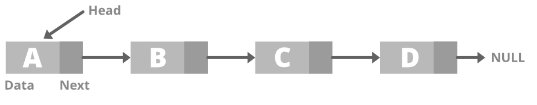
\includegraphics[width=0.75\textwidth]{imagenes/Lista individualmente vinculada.png}
        \caption{Pie de pagina.}
        \label{fig:individual}
    \end{figure}

    \item \textbf{Lista doblemente enlazada:} En una lista doblemente enlazada, tiene dos referencias, una al nodo siguiente y otra al nodo anterior.
    \begin{figure}[h]
        \centering
        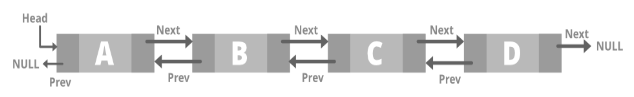
\includegraphics[width=0.75\textwidth]{imagenes/Lista doblemente enlazada.png}
        \caption{Pie de pagina.}
        \label{fig:doblemente}
    \end{figure}

\end{enumerate}

\section*{Forma para crear un LinkedList}
Se debe tomar en cuenta que para su creacion se debe importar la biblioteca:

\begin{center}
    import java.util.LinkedList;
\end{center}
A continuacion se presenta la forma para declarar un LinkedList:

\begin{center}
    $LinkedList<[Tipo de dato]> [Identificador] = new LinkedList<[Tipo de dato]>([Tamano]);$
\end{center}
Donde se tiene que:
\begin{itemize}
    \item \textbf{Tipo de dato:} se definira el tipo de dato contendra cada uno de los elementos de la LinkedList.
    \item \textbf{Identificador:} se definira su nombre.
    \item \textbf{Tamano:} se le designara el tamano que tendra.
\end{itemize}

\section*{Metodos principales en Linked List}
\begin{itemize}
    \item \textbf{add(Objeto):} Nos permite agregar un elemento al final de LinkedList.
    
    \item \textbf{add(int index, Object):} Permite agregar un elemento en un indice en especifico en LinkedList.
    
    \lstset{language = Java, breaklines=true, basicstyle=\footnotesize}
    Ejemplo:
    \begin{lstlisting}[frame=single]
    LinkedList<String> LL = new LinkedList<>();

    LL.add("Hola");  
    LL.add(1, "Mundo");
    \end{lstlisting}
    
    \item \textbf{get():} Nos permite buscar o recuperar un elemento de un indice en especifico de LinkedList. Como parametros se le da el indice del elemento que deseamos obtener. Este retorna el elemento encontrado en esa posicion.
    
    Ejemplo:
    \lstset{language = Java, breaklines=true, basicstyle=\footnotesize}
    \begin{lstlisting}[frame=single]
    LinkedList<String> list = new LinkedList<String>();

    list.add("Esto");
    list.add(" es");
    list.add(" una prueba");
    list.add(" 10");

    System.out.println("El elemento en la posicion 2 es: "+ list.get(2));
    \end{lstlisting}
    
    \item \textbf{set():} Dado que una LinkedList esta indexada, el elemento que deseamos cambiar esta referenciado por el indice del elemento. Por lo tanto, este metodo toma un indice y el elemento actualizado que debe insertarse en ese indice.

    Ejemplo:
    \lstset{language = Java, breaklines=true, basicstyle=\footnotesize}
    \begin{lstlisting}[frame=single]
    LinkedList<String> LL = new LinkedList<>();

    LL.add("Hola");  
    LL.add(1, "Mundo");

    ll.set(1, "a todos");
    \end{lstlisting}
    
    \item \textbf{remove(Object):} Este metodo se utiliza para eliminar un objeto de LinkedList. De forma que si hay varios objetos de este tipo, se elimina la primera aparicion del objeto mandado como parametro.
    
    \item \textbf{remove(int index):} Dado que una LinkedList esta indexada, este metodo toma un valor entero que simplemente elimina el elemento presente en ese indice especifico en LinkedList. Despues de eliminar el elemento, todos los elementos se mueven hacia la izquierda para llenar el espacio y se actualizan los indices de los objetos.

    Ejemplo:
    \lstset{language = Java, breaklines=true, basicstyle=\footnotesize}
    \begin{lstlisting}[frame=single]
    LinkedList<String> LL = new LinkedList<>();

    LL.add("Hola");  
    LL.add(" a");
    LL.add(" todos :)");

    LL.remove(1);
    LL.remove(" todos");
    \end{lstlisting}
    
    \item \textbf{contains():}Se utiliza para verificar si un elemento se encuentra dentro de una LinkedList creada. De forma que toma el elemento como parametro, devuelve verdadero si el elemento se encuentra, en caso contrario, devuelve falso.

    Ejemplo:
    \lstset{language = Java, breaklines=true, basicstyle=\footnotesize}
    \begin{lstlisting}[frame=single]
    LinkedList<String> LL = new LinkedList<>();

    LL.add("Hola");  
    LL.add( " a");
    LL.add( " todos :)");

    if(LL.contains("Hola") == true){
        System.out.println("El elemento 'Hola' se encuentra en la lista :) ");
    }
    else{
    	System.out.println("El elemento no esta en la lista :( ");
    }
    \end{lstlisting}
    
    \item \textbf{peek():} Examina el elemento que se encuentra en el encabezado de la lista, se forma que se recupera mas no se elimina.
    
    \item \textbf{peekFirst():} Similar al metodo anterior, recupera el primer elemento de esta lista, o devuelve nulo si la lista se encuentra vacia.
    
    \item \textbf{peekLast():} Nos permite recuperar el ultimo elemento que se encuentre en la lista, o devuelve nulo si la lista se encuentra vacia.

    Ejemplo:
    \lstset{language = Java, breaklines=true, basicstyle=\footnotesize}
    \begin{lstlisting}[frame=single]
    LinkedList<String> LL = new LinkedList<>();

    LL.add("Hola");  
    LL.add( " a");
    LL.add( " todos :)");

    System.out.println("Encabezado de la lista: " +LL.peek());

    System.out.println("Primer elemento de la lista: " +LL.peekFirst());

    System.out.println("Ultimo elemento de la lista: " + LL.peekLast());
    \end{lstlisting}

    \item \textbf{clone():} Se utiliza para crear una copia superficial de la lista vinculada. No necesita de un parametro para su funcionamiento, puesto que solo devuelve una copia de la instancia de la lista.

    Ejemplo:
    \lstset{language = Java, breaklines=true, basicstyle=\footnotesize}
    \begin{lstlisting}[frame=single]
    LinkedList<String> list = new LinkedList<String>();

    list.add("Esto");
    list.add(" es");
    list.add(" una prueba");
    list.add(" 10");

    LinkedList sec_list = new LinkedList();

    sec_list = list.clone();
    \end{lstlisting}
    
\end{itemize}

\section{Vectores (Vector):}
Para el caso de los vectores, estos llegan a ser semejantes a las matrices, donde en ellos se puede acceder a los elementos del objeto vectorial, esto por medio de un indice en el vector. Como tal, el vector implementa una matriz dinamica, como tambien, dicho vector no limita su tamano.

Si nos damos cuenta, el vector es similar a ArrayList, pero con 2 diferencias:
\begin{enumerate}
    \item El vector esta sincronizado.
    \item El vector contiene muchos metodos heredados que no forman parte del marco de las colecciones.
\end{enumerate}

\begin{figure}[h]
    \centering
    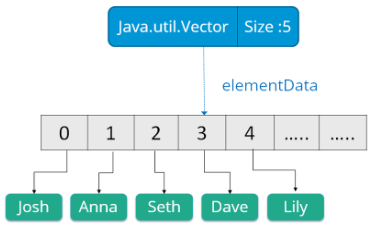
\includegraphics[width=0.75\textwidth]{imagenes/Ejemplo Grafico Vector.png}
    \caption{Pie de pagina.}
    \label{fig:vector}
\end{figure}

\section*{Forma para crear un Vector}
Se debe tomar en cuenta que para su creacion se debe importar la biblioteca:
\begin{center}
    import java.util.Vector;
\end{center}
A continuacion se presenta la forma para declarar un LinkedList:
\begin{center}
    $Vector<[Tipo de dato]> [Identificador] = new Vector<[Tipo de dato]>([Tamano]);$
\end{center}

Donde se tiene que:
\begin{itemize}
    \item \textbf{Tipo de dato:} se definira el tipo de dato contendra cada uno de los elementos del Vector.
    \item \textbf{Identificador:} se definira su nombre.
    \item \textbf{Tamano:} se le designara el tamano que tendra.
\end{itemize}

\section*{Metodos principales de Vector}
\begin{itemize}
    \item \textbf{add():} Nos permite anadir un elemento especificado al final de un vector creado, todo esto mediante el aumento del tamano del vector por 1.

    \item \textbf{add(int index, Object):} El metodo inserta un elemento en un indice especificado en el vector, de forma que desplaza el elemento que se encuentra actualmente en esa posicion, y cualquier elemento posterior a la derecha.

    Ejemplo:
    \lstset{language = Java, breaklines=true, basicstyle=\footnotesize}
    \begin{lstlisting}[frame=single]
    Vector<String> vec_tor = new Vector<String>();

    vec_tor.add("Hola, ");
    vec_tor.add("esto es ");
    vec_tor.add("otra prueba :) ");
    vec_tor.add(1, " . Como estas? ");
    \end{lstlisting}

    \item \textbf{clear():} Se utiliza para eliminar todos los elementos de un vector, es necesario mencionar que el metodo solo borra los elementos mas no el vector.

    Ejemplo:
    \lstset{language = Java, breaklines=true, basicstyle=\footnotesize}
    \begin{lstlisting}[frame=single]
    Vector<String> vec_tor = new Vector<String>();

    vec_tor.add("Hola, ");
    vec_tor.add("esto es ");
    vec_tor.add("otra prueba :) ");

    vec_tor.clear();

    System.out.println("El vector se encuentra vacio: " + vec_tor);
    \end{lstlisting}

    \item \textbf{remove():} Nos permite eliminar un elemento de un vector mediante una posicion o indice dado.

    Ejemplo:
    \lstset{language = Java, breaklines=true, basicstyle=\footnotesize}
    \begin{lstlisting}[frame=single]
    Vector<String> vec_tor = new Vector<String>();

    vec_tor.add("Hola, ");
    vec_tor.add("esto es ");
    vec_tor.add("otra prueba :) ");

    vec_tor.remove(2);
    \end{lstlisting}

    \item \textbf{contains():} Nos permite verificar si un elemento en especifico se encuentra en el vector. Como parametros se le da un elemento del tipo de vector por buscar. Retorna verdadero en caso de encontrar el elemento, caso contrario devuelve falso.

    Ejemplo:
    \lstset{language = Java, breaklines=true, basicstyle=\footnotesize}
    \begin{lstlisting}[frame=single]
    Vector<String> vec_tor = new Vector<String>();

    vec_tor.add("Bienvenidos ");
    vec_tor.add("sean ");
    vec_tor.add("todos ");

    if(vec_tor.contains(":)") == true){
        System.out.println("El elemento esta en el vector :) ");
    }
    else{
	   System.out.println("El elemento no esta en el vector :( ");
    }
    \end{lstlisting}

    \item \textbf{size():} Se utiliza para conocer el tamano o el numero de elementos presentes en el vector. No necesita de un parametro para su funcionamiento. Retorna el tamano o la cantidad de elementos en el vector.

    Ejemplo:
    \lstset{language = Java, breaklines=true, basicstyle=\footnotesize}
    \begin{lstlisting}[frame=single]
    Vector<Integer> vec_tor = new Vector<Integer>();

    vec_tor.add(15);
    vec_tor.add(4);
    vec_tor.add(98);
    vec_tor.add(32);

    System.out.println("Tamano del vector:  " + vec_tor.size());
    \end{lstlisting}
    
    \item \textbf{indexOfObject():} Nos permite verificar y encontrar la ocurrencia de un elemento dentro del vector. Como parametro se envia el elemento del tipo vector. Si el elemento esta presente, se devuelve el indice de su primera aparicion en el vector, en caso contrario devuelve -1.
    
    Ejemplo:
    \lstset{language = Java, breaklines=true, basicstyle=\footnotesize}
    \begin{lstlisting}[frame=single]
    Vector<Integer> vec_tor = new Vector<Integer>();

    vec_tor.add(15);
    vec_tor.add(4);
    vec_tor.add(98);
    vec_tor.add(32);
    vec_tor.add(4);

    System.out.println("Indice de la primera aparicion del elemento 4: :"+ vec_tor.indexOf(4));
    \end{lstlisting}
\end{itemize}

\section*{Stack (Pila):}
En el marco de Java Collection, se proporciona la clase Stack (Pila) que modela e implementa una estructura de datos Stack. Un Stack es una estructura de datos lineal que solo tienen un unico punto de acceso fijo por el cual se anaden, eliminan o se consultan elementos. El modo de acceso a los elementos es de tipo LIFO ( Last In First Out, ultimo en entrar, primero en salir).

Tambien se puede decir que la clase extiende Vector y trata la clase como una pila, de esta manera, la clase tambien puede denominarse subclase de Vector.
\section*{Forma para crear un Stack}
Se debe tomar en cuenta que para su creacion se debe importar la biblioteca:

\begin{center}
    import java.util.*;
\end{center}

Para este caso en particular donde la clase Stack, se deriva de la clase Vector, se debe realizar lo siguiente:
\begin{center}
    $public class Stack<E> extends Vector<E>$
\end{center}
A continuacion se presenta la forma para declarar un Stack:
\begin{center}
    $Stack<[Tipo de dato]> [Identificador] = new Stack<[Tipo de dato]>([Tamano]);$
\end{center}
Donde se tiene que:
\begin{itemize}
    \item \textbf{Tipo de dato:} se definira el tipo de dato contendra cada uno de los elementos del Stack
    \item \textbf{Identificador:} se definira su nombre.
    \item \textbf{Tamano:} se le designara el tamano que tendra.
\end{itemize}

\section*{Metodos principales de Stack}
\begin{itemize}
    \item \textbf{push():} Permite agregar un elemento a la pila, de forma que coloca el elemento en la parte superior de la pila. Como parametro acepta un elemento de tipo Pila y se refiere al elemento del cual sera insertado.

    Ejemplo:
    \lstset{language = Java, breaklines=true, basicstyle=\footnotesize}
    \begin{lstlisting}[frame=single]
    Stack<String> pila = new Stack<String>();

    pila.push("Hola ");
    pila.push("esto es ");
    pila.push("una prueba :) ");

    System.out.print(pila);
    \end{lstlisting}

    \item \textbf{search():} Permite buscar un elemento dentro de la pila, de tal forma que se obtiene su distancia desde la parte superior. Como parametro se ingresa el elemento del cual se buscara. El metodo devuelve la posicion del elemento si se encuentra en la pila, en caso de no encontrarlo, se devolvera un -1.

    Ejemplo:
    \lstset{language = Java, breaklines=true, basicstyle=\footnotesize}
    \begin{lstlisting}[frame=single]
    Stack<String> pila = new Stack<String>();

    pila.push("Hola ");
    pila.push("esto es ");
    pila.push("una prueba :) ");

    System.out.println("Posicion del elemento 'Hola':  "+pila.search("Hola"));
    \end{lstlisting}

    \item \textbf{pop():} Permite extraer un elemento de la pila. El elemento se saca de la parte superior de la pila y se quita de la misma. El metodo no necesita de un parametro para su funcionamiento. De esta forma, devuelve el elemento del cual sera quitado, para posteriormente eliminarlo de la pila.
    
    Ejemplo:
    \lstset{language = Java, breaklines=true, basicstyle=\footnotesize}
    \begin{lstlisting}[frame=single]
    Stack<String> pila = new Stack<String>();

    pila.push("Hola ");
    pila.push("esto es ");
    pila.push("una prueba :) ");

    System.out.println("Se ha quitado el elemento: "+pila.pop());

    System.out.print(pila);
    \end{lstlisting}

    \item \textbf{empty():} Permite verificar si una pila esta vacia o no. El metodo es de tipo booleano y devuelve verdadero si la pila esta vacia, de lo contrario, devolvera falso.

    Ejemplo:
    \lstset{language = Java, breaklines=true, basicstyle=\footnotesize}
    \begin{lstlisting}[frame=single]
    Stack<String> pila = new Stack<String>();

    System.out.println("La pila se encuentra vacia? "+pila.empty());
    \end{lstlisting}
\end{itemize}

\section{Colecciones de Java: Cola (Queue)}
En Java, la estructura de Cola ordena los elementos de la manera FIFO (First In, First Out o Primero en entrar, Primero en salir). En la Cola, el primer elemento ingresado se elimina primero, y el ultimo se elimina al final.

Los metodos basicos de la Cola existe de 2 formas:
\begin{enumerate}
    \item Se lanza una excepcion si se falla la operacion.
    \item Devuelve un valor especial.
\end{enumerate}
\begin{figure}[h]
    \centering
    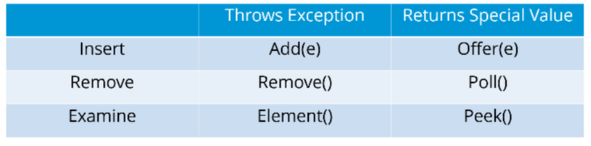
\includegraphics[width=0.75\textwidth]{imagenes/Metodos basicos de la Cola .png}
    \caption{Pie de pagina.}
    \label{fig:tabla}
\end{figure}
Para este caso en cuestion, la cola prioridad se implementa en la interfaz de Cola, de esta manera, cada elemento se ordena de acuerdo con su orden natural, o por un comparador proporcionado en el momento de la construccion de la cola.

\section*{Forma para crear un Queue}
Se debe tomar en cuenta que para su creacion se debe importar la biblioteca:
\begin{center}
    import java.util.Queue;
\end{center}
A continuacion se presenta la forma para declarar un LinkedList:
\begin{center}
    $Queue<[Tipo de dato]> [Identificador] = new Queue<[Tipo de dato]>([Tamano]);$
\end{center}
Donde se tiene que:
\begin{itemize}
    \item \textbf{Tipo de dato:} se definira el tipo de dato contendra cada uno de los elementos del Queue.
    \item \textbf{Identificador:} se definira su nombre.
    \item \textbf{Tamano:} se le designara el tamano que tendra.
\end{itemize}

\section*{Metodos principales de Cola (Queue)}
\begin{itemize}
    \item \textbf{add():} Inserta un elemento pasado en el parametro al final de la cola en caso de haber espacio. Si la cola al momento de insertar un elemento se encuentra en su capacidad limite, devolvera una excepcion. 
    
    Ejemplo:
    \lstset{language = Java, breaklines=true, basicstyle=\footnotesize}
    \begin{lstlisting}[frame=single]
    Queue<Integer> cola = new LinkedList<Integer>();

    cola.add(444);
    cola.add(356);
    cola.add(890);

    System.out.println("Cola: " +cola);
    \end{lstlisting}

    \item \textbf{offer():} Permite insertar un el elemento especificado en la cola si es posible hacerlo inmediatamente sin violar las restricciones de su capacidad. Este metodo es preferible al metodo add(), ya que este metodo no lanza una excepcion cuando la capacidad del contenedor esta llena, puesto que solo devuelve un falso.
    
    Ejemplo:
    \lstset{language = Java, breaklines=true, basicstyle=\footnotesize}
    \begin{lstlisting}[frame=single]
    Queue<Integer> cola = new LinkedList<Integer>(3);

    cola.add(444);
    cola.add(356);
    cola.add(890);

    if(cola.offer(250)){
        System.out.println("Se ha insertado el elemento 250 en la cola :) ");
    }
    else{
    	System.out.println("La cola se encuentra llena :( ");
    }
    \end{lstlisting}

    \item \textbf{remove():} Devuelve y elimina el elemento al frente de la cola. El metodo regresa una excepcion en caso de que la cola este vacia.
    
    Ejemplo:
    \lstset{language = Java, breaklines=true, basicstyle=\footnotesize}
    \begin{lstlisting}[frame=single]
    Queue<Integer> cola = new LinkedList<Integer>();

    cola.add(444);
    cola.add(356);
    cola.add(890);
    cola.add(777);

    System.out.println("Elemento eliminado de la cabeza de la cola: " + cola.remove());
    \end{lstlisting}

    \item \textbf{poll():} Similar al metodo anterior, devuelve y elimina el elemento al frente de la cola. La diferencia de este metodo respecto a remove(), se debe a que este no lanza una excepcion cuando la cola esta vacia, en su lugar devuelve un valor nulo.
    
    Ejemplo:
    \lstset{language = Java, breaklines=true, basicstyle=\footnotesize}
    \begin{lstlisting}[frame=single]
    Queue<Integer> cola = new LinkedList<Integer>();

    cola.add(444);
    cola.add(356);
    cola.add(890);
    cola.add(777);

    System.out.println("Elemento eliminado de la cabeza de la cola: " + cola.poll());
    \end{lstlisting}

    \item \textbf{element():} Devuelve el elemento que se encuentre al frente de la cola, es necesario mencionar que dicho elemento no lo elimina. Su funcionamiento es semejante a peek(), pero su diferencia radica en que solo lanza una excepcion si la cola esta vacia.
    
    Ejemplo:
    \lstset{language = Java, breaklines=true, basicstyle=\footnotesize}
    \begin{lstlisting}[frame=single]
    Queue<Integer> cola = new LinkedList<Integer>();

    cola.add(444);
    cola.add(356);
    cola.add(890);
    cola.add(777);
    
    System.out.println("Elemento en la cabeza de la cola: " + cola.element());
    \end{lstlisting}
\end{itemize}

\section{Colecciones de Java: Conjuntos (Sets)}
Un conjunto se refiere a una coleccion que no puede contener elementos duplicados. Su uso se enfoca principalmente en modelar la abstraccion de conjuntos matematicos. Para este caso Set tiene su implementacion en varias clases como:
\begin{enumerate}
    \item \textbf{Hashsests}
    \item \textbf{LinkedHashet}
    \item \textbf{TreeSet}
\end{enumerate}

\section*{HashSet}
En Java, la clase HashSet crea una coleccion que usa una tabla hash para su almacenamiento. HashSet solo puede contener elementos unicos, a su vez, hereda la clase AbstractSet e implementa la interfaz Set.

\section*{Forma para crear un HashSet}
Se debe tomar en cuenta que para su creacion se debe importar la biblioteca:
\begin{center}
    import java.util.HashSet;
\end{center}
A continuacion se presenta la forma para declarar un HashSet:
\begin{center}
   $HashSet<[Tipo de dato]> [Identificador] = new HashSet<[Tipo de dato]>([Tamano]);$ 
\end{center}
Donde se tiene que:
\begin{itemize}
    \item \textbf{Tipo de dato:} se definira el tipo de dato contendra cada uno de los elementos del HashSet.
    \item \textbf{Identificador:} se definira su nombre.
    \item \textbf{Tamano:} se le designara el tamano que tendra.
\end{itemize}

\section*{Metodos principales de Hashset}
\begin{itemize}
    \item \textbf{add():} Permite anadir o insertar elementos al Hashset, sin embargo, la orden de insercion no se conserva. Es necesario tener en cuenta que los elementos duplicados no estan permitidos, por lo que cada elemento duplicado que se encuentre se ignorara. 

    Ejemplo:
    \lstset{language = Java, breaklines=true, basicstyle=\footnotesize}
    \begin{lstlisting}[frame=single]
    HashSet<String> hs = new HashSet<String>();

    hs.add("A");
    hs.add("B");
    hs.add("C");
    hs.add("D");
    \end{lstlisting}

    \item \textbf{contains():} Verifica si un elemento especifico se encuentra dentro del HashSet. Como parametro se envia un elemento del tipo HashSet. Retorna  verdadero si el elemento se encuentra, en caso contrario devuelve falso.

    Ejemplo:
    \lstset{language = Java, breaklines=true, basicstyle=\footnotesize}
    \begin{lstlisting}[frame=single]
    HashSet<String> hs = new HashSet<String>();

    hs.add("A");
    hs.add("B");
    hs.add("C");
    hs.add("D");

    if(hs.contains("D") == true){
        System.out.println("La letra 'D' esta presente :) ");
    }
    else{
	   System.out.println("La letra 'D' no esta :( ");
    }
    \end{lstlisting}

    \item \textbf{clear():} Permite eliminar todos los elementos de un HashSet. El uso de este metodo solo borra todos los elementos del conjunto, mas no elimina al conjunto.

    Ejemplo:
    \lstset{language = Java, breaklines=true, basicstyle=\footnotesize}
    \begin{lstlisting}[frame=single]
    HashSet<String> hs = new HashSet<String>();

    hs.add("A");
    hs.add("B");
    hs.add("C");
    hs.add("D");

    System.out.println("Conjunto despues de usar clear(): " + hs.clear());
    \end{lstlisting}

    \item \textbf{isEmpty():} Permite verificar si un Hashset se encuentra vacio. Este devuelve verdadero si el HashSet esta vacio, en caso contrario devolvera un falso.

    Ejemplo:
    \lstset{language = Java, breaklines=true, basicstyle=\footnotesize}
    \begin{lstlisting}[frame=single]
    HashSet<String> hs = new HashSet<String>();

    hs.add("A");
    hs.add("B");
    hs.add("C");
    hs.add("D");

    if(hs.isEmpty() == true){
        System.out.println("El conjunto esta vacio :) ");
    }
    else{
    	System.out.println("El conjunto tiene elementos :( ");
    }
    \end{lstlisting}

    \item \textbf{remove():} Permite eliminar un elemento especificado dentro del HashSet.

    Ejemplo:
    \lstset{language = Java, breaklines=true, basicstyle=\footnotesize}
    \begin{lstlisting}[frame=single]
    HashSet<String> hs = new HashSet<String>();

    hs.add("A");
    hs.add("B");
    hs.add("C");
    hs.add("D");

    hs.remove("D");
    \end{lstlisting}

    \item \textbf{clone():} Se utiliza para devolver una copia superficial del conjunto de hash. No necesita de ningun parametro para su funcionamiento.

    Ejemplo:
    \lstset{language = Java, breaklines=true, basicstyle=\footnotesize}
    \begin{lstlisting}[frame=single]
    HashSet<Integer> hs = new HashSet<Integer>();

    hs.add(1);
    hs.add(2);
    hs.add(3);
    hs.add(4);

    HashSet hs_2  = new HashSet();

    hs_2 = hs.clone();

    System.out.println("Nuevo conjunto clonado: " +hs_2);
    \end{lstlisting}

    \item \textbf{size():} Permite obtener el tamano, o conocer la cantidad de elementos que se encuentran en el HashSet.

    Ejemplo:
    \lstset{language = Java, breaklines=true, basicstyle=\footnotesize}
    \begin{lstlisting}[frame=single]
    HashSet<Integer> hs = new HashSet<Integer>();

    hs.add(1);
    hs.add(2);
    hs.add(3);
    hs.add(4);

    System.out.println("Tamano del conjunto: " +hs.size());
    \end{lstlisting}
\end{itemize}

\section*{LinkedHashSet (HashSet vinculado)}
En Java, HashSet vinculado o LinkedHashSet es una tabla Hash con una implementacion de lista vinculada de la interfaz Set. Contiene elementos unicos como HashSet, tambien, proporciona cada uno de los metodos HashSet, manteniendo el orden de insercion.

\section*{Forma para crear un LinkedHashSet}
Se debe tomar en cuenta que para su creacion se debe importar la biblioteca:
\begin{center}
    import java.util.LinkedHashSet;
\end{center}
A continuacion se presenta la forma para declarar un LinkedHashSet:
\begin{center}
    $LinkedHashSet<[Tipo de dato]> [Identificador] = new LinkedHashSet<[Tipo de dato]>([Tamano]);$
\end{center}
Donde se tiene que:
\begin{itemize}
    \item \textbf{Tipo de dato:} se definira el tipo de dato contendra cada uno de los elementos del LinkedHashSet.
    \item \textbf{Identificador:} se definira su nombre.
    \item \textbf{Tamano:} se le designara el tamano que tendra.
\end{itemize}

\section*{TreeSet}
La clase TreeSet implementa la interfaz Set, del cual usa un arbol binario para su almacenamiento. Cada uno de los objetos se almacenan en orden ascendente. Dicha clase hereda la clase AbstractSet e implementa la interfaz NavigableSet. Al igual que las anteriores clases, este solo puede contener elementos unicos. La clase TreeSet llega a ser mucho mas rapida en el tiempo de acceso y recuperacion de los elementos.

\section*{Forma para crear un TreeSet}
Se debe tomar en cuenta que para su creacion se debe importar la biblioteca:
\begin{center}
    import java.util.Set;
\end{center}
A continuacion se presenta la forma para declarar un TreeSet:
\begin{center}
    $Set<[Tipo de dato]> [Identificador] = new TreeSet<[Tipo de dato]>([Tamano]);$
\end{center}
Donde se tiene que:
\begin{itemize}
    \item \textbf{Tipo de dato:} se definira el tipo de dato contendra cada uno de los elementos del TreeSet.
    \item \textbf{Identificador:} se definira su nombre.
    \item \textbf{Tamano:} se le designara el tamano que tendra.
\end{itemize}

\section*{Metodos principales de TreeSet}
\begin{itemize}
    \item \textbf{add():} Permite agregar un elemento en especifico dentro de un TreeSet. El metodo agrega al elemento solo si el elemento no se encuentra, caso contrario el metodo devuelve un falso.
    
    \item \textbf{addAll():} Permite agregar todos los elementos de la coleccion al conjunto creado. Cada uno de los elementos se agregan aleatoriamente sin seguir ningun orden especifico.
    
    Ejemplo:
    \lstset{language = Java, breaklines=true, basicstyle=\footnotesize}
    \begin{lstlisting}[frame=single]
    TreeSet<String> tree = new TreeSet<String>();

    tree.add("Hola ");
    tree.add("esto es ");
    tree.add("una prueba ");

    TreeSet<String> tree_2 = new TreeSet<String>();

    tree_2.add("Bienvenidos ");
    tree_2.add("sean todos ");

    tree.addAll(tree_2);

    System.out.println("TreeSet: " + tree);
    \end{lstlisting}

    \item \textbf{contains():} Se utiliza para comprobar si un elemento especifico esta presente en el TreeSet. Devuelve verdadero si el elemento se encuentra dentro del TreeSet, en caso contrario devuelve un falso.

    \item \textbf{containsAll():} Permite comprobar si dos conjuntos contienen los mismos elementos o no. Toma un conjunto como parametro y devuelve verdadero si todos los elementos de este conjunto estan presentes en el otro conjunto.
    
    Ejemplo:
    \lstset{language = Java, breaklines=true, basicstyle=\footnotesize}
    \begin{lstlisting}[frame=single]
    TreeSet<Integer> set = new TreeSet<Integer>();

    set.add(12);
    set.add(99);
    set.add(42);
    set.add(30);

    System.out.println("El conjunto contiene al 99? "+ set.contains(99));

    TreeSet<Integer> set_2 = new TreeSet<Integer>();

    set_2.add(12);
    set_2.add(99);
    set_2.add(42);
    set_2.add(30);

    System.out.println("El conjunto 1 contiene al conjunto 2?  "+ set.containsAll(set_2));
    \end{lstlisting}

    \item \textbf{isEmpty():} Permite comprobar y verificar si un TreeSet se encuentra vacio. Retorna verdadero si el TreeSet esta vacio, en caso contrario devuelve falso.
    
    Ejemplo:
    \lstset{language = Java, breaklines=true, basicstyle=\footnotesize}
    \begin{lstlisting}[frame=single]
    TreeSet<String> tree = new TreeSet<String>();

    if(tree.isEmpty() == true){
        System.out.println("El conjunto esta vacio :) ");
    }
    else{
	   System.out.println("El conjunto tiene elementos :( ");
    }
    \end{lstlisting}

    \item \textbf{remove():} Permite eliminar un elemento en particular de un TreeSet. Como parametros se le da el elemento del cual se eliminara del conjunto. Retorna verdadero si se elimina el elemento dado del conjunto, de lo contrario devuelve falso.
    
    Ejemplo:
    \lstset{language = Java, breaklines=true, basicstyle=\footnotesize}
    \begin{lstlisting}[frame=single]
    TreeSet<Integer> set = new TreeSet<Integer>();

    set.add(12);
    set.add(99);
    set.add(42);
    set.add(30);

    sett.remove(42);

    System.out.println("Nuevo conjunto despues de haber eliminado el elemento 42: "+set);
    \end{lstlisting}

    \item \textbf{clear():} Permite eliminar todos los elementos de un TreeSet. Al usar este metodo borra unicamente los elementos del conjunto, mas no el conjunto.

    Ejemplo:
    \lstset{language = Java, breaklines=true, basicstyle=\footnotesize}
    \begin{lstlisting}[frame=single]
    TreeSet<Integer> set = new TreeSet<Integer>();

    set.add(12);
    set.add(99);
    set.add(42);
    set.add(30);

    set.clear();

    System.out.println("Conjunto despues haber eliminado sus elementos: "+set);
    \end{lstlisting}

    \item \textbf{clone():} Devuelve una copia superficial del conjunto de arboles.

    Ejemplo:
    \lstset{language = Java, breaklines=true, basicstyle=\footnotesize}
    \begin{lstlisting}[frame=single]
    TreeSet<String> tree = new TreeSet<String>();

    tree.add("Hola ");
    tree.add("esto es ");
    tree.add("una prueba ");

    TreeSet tree_2 = new TreeSet();

    tree_2 = tree.clone();

    System.out.println("Conjunto clonado: "+tree_2);
    \end{lstlisting}

    \item \textbf{fist():} Permite devolver el primero de los elementos de un TreeSet. El primer elemento aqui se refiere al mas bajo de los elementos del conjunto, puesto que nos encontramos en un conjunto de arboles. Es necesario mencionar que si los elementos son de tipo entero, se devuelve el numero entero mas pequeno; en caso de ser elementos de tipo string, los elementos se verifican en orden alfabetico.

    \item \textbf{last():} Permite devolver el ultimo elemento de un TreeSet. El ultimo elemento aqui se refiere al mas alto de los elementos del conjunto. Es necesario mencionar que si los elementos son de tipo entero, se devuelve el entero mas grande; en caso de ser elementos de tipo string, los elementos se verifican en orden alfabetico

    Ejemplo:
    \lstset{language = Java, breaklines=true, basicstyle=\footnotesize}
    \begin{lstlisting}[frame=single]
    TreeSet<Integer> tree = new TreeSet<Integer>();

    tree.add(500);
    tree.add(12);
    tree.add(210);
    tree.add(98);
    tree.add(7);

    System.out.println("El primer elemento del conjunto es: "+tree.first());

    System.out.println("El ultimo elemento del conjunto es: "+tree.last());
    \end{lstlisting}

    \item \textbf{size():} Nos permite obtener el tamano del conjunto de arboles, o la cantidad de elementos presentes en el. No necesita de un parametro para su funcionamiento.

    Ejemplo:
    \lstset{language = Java, breaklines=true, basicstyle=\footnotesize}
    \begin{lstlisting}[frame=single]
    TreeSet<Integer> tree = new TreeSet<Integer>();

    tree.add(500);
    tree.add(12);
    tree.add(210);
    tree.add(98);
    tree.add(7);

    System.out.println("Tamano del conjunto: "+tree.size());
    \end{lstlisting}
\end{itemize}

\section*{Referencias electronicas:}
\begin{itemize}
    \item ArrayList en Java – Acervo Lima. (s. f.). Recuperado 24 de septiembre de 2022, de \href{https://bit.ly/3fB4HAN}{https://es.acervolima.com/arraylist-en-java/}
    
    \item Clase de vector en Java – Acervo Lima. (s. f.). Recuperado 24 de septiembre de 2022, de \href{https://es.acervolima.com/clase-de-vector-en-java-1/}{https://es.acervolima.com/clase-de-vector-en-java-1/}
    
    \item COLECCIONES JAVA: INTERFAZ, LISTA, COLA, CONJUNTOS EN JAVA CON EJEMPLOS - BLOG. (s. f.). Recuperado 24 de septiembre de 2022, de \href{https://es.quish.tv/java-collections-interface}{https://es.quish.tv/java-collections-interface}
    
    \item Interfaz de cola en Java – Acervo Lima. (s. f.). Recuperado 24 de septiembre de 2022, de \href{https://es.acervolima.com/interfaz-de-cola-en-java/}{https://es.acervolima.com/interfaz-de-cola-en-java/}
    
    \item LinkedList en Java – Acervo Lima. (s. f.). Recuperado 24 de septiembre de 2022, de \href{https://es.acervolima.com/linkedlist-en-java-1/}{https://es.acervolima.com/linkedlist-en-java-1/}
\end{itemize}

\end{document}